% !TEX root = _yoko-pbl2026.tex

% ==========================================
% プロジェクト予稿（1P）の本文
% ==========================================

\section{はじめに}
近年，デジタル技術の発展により，音楽と映像を組み合わせた表現は多様化しており，
ライブパフォーマンスにおいても，音楽の進行に応じて映像が変化する演出が広く用いられている．
視覚情報と聴覚情報の統合は，観客の知覚や感情体験に大きな影響を与えることが指摘されており，
音楽と映像の適切な組み合わせが没入感を高める要因となることが示されている\cite{asano}．
一方で，映像演出には専門的な知識や操作を要する場合が多く，
演奏者自身が演奏中に直感的に映像を制御できるシステムは十分に検討されていない．

そこで本研究では，ピアノ演奏に基づいて映像をリアルタイムに制御・生成するシステムを
構築する．MIDIキーボードから取得した演奏情報およびフットペダル入力を用い，
TouchDesigner\cite{TouchDesigner}上で映像表現を制御する．また，生成AIを用いて楽曲の歌詞や雰囲気に
応じた映像素材を生成し，静止画や動画として演出に取り入れる．
本システムは，従来の音楽特徴量のみに基づく自動同期ではなく，演奏者自身の判断による
操作を可能とすることで，演奏の即興性や音楽的意図を映像表現に反映できる点に特徴がある．

%2------*------*------*------*------*------*------*------*------*------*------*
\section{ピアノ演奏に基づく映像制御手法}
%2.1
\subsection{システム概要}
本研究では，ピアノ演奏の情報を入力として映像演出をリアルタイムに制御する手法を提案する．
本手法は，演奏者の演奏行為そのものを映像操作のトリガとすることで，演奏と映像が自然に
同期した表現を実現することを目的としている．

本システムは，演奏情報を取得する入力部，取得した情報を処理して映像制御信号を生成する
制御部，および映像を生成・合成・出力する映像生成部から構成される．これらの各処理は
リアルタイムで連携して動作し，演奏中の入力が即座に映像表現へ反映される．

ピアノ演奏の入力にはMIDIキーボードを用い，ノート番号およびベロシティ情報を取得する．
ノート番号は鍵盤位置に対応した映像要素の制御に用いられ，ベロシティ情報は演奏の強弱に
応じたエフェクトの大きさや発光強度などのパラメータ制御に利用される．これらの情報を
もとに，TouchDesigner上で映像エフェクトの発生や強度を制御する．具体的には，鍵盤入力に
応じて発光や炎，煙などの視覚エフェクトを生成し，演奏の強弱や時間的変化を視覚的に表現する．
さらに，本手法ではUSBフットペダルを併用し，演奏中に映像素材や演出パターンを切り替える
仕組みを導入した．フットペダル操作は演奏中の足による入力を前提としており，手を使うこと
なく映像制御を行うことができる．これにより，歌詞表示の切り替えや情景映像の変更などを，
演奏への集中を妨げることなく実行できる．
映像素材には，生成AIを用いて事前に作成した画像を使用し，楽曲の歌詞やイメージに基づいた
視覚表現を行う．歌詞を含む楽曲については，歌詞データを入力として生成した画像を映像素材
として用い，楽曲内容と対応した視覚的演出を実現する．生成された画像および歌詞データは
TouchDesignerに取り込まれ，演奏状況に応じてリアルタイムに合成・表示される．

以上の構成により，本システムは時間や楽譜進行に基づく自動同期ではなく，演奏者の判断に基づいて
映像を制御する点に特徴がある．これにより，即興性や表現の自由度を保ったまま，音楽と映像が
一体となったライブパフォーマンス環境を構築した．

%2.2
\subsection{実演について}

本システムを用いたデモ演奏とともに，ゼミ生8名を対象とした簡易的なテスト演奏を実施し，
ピアノ演奏中の指定箇所においてUSBフットペダルを操作させた．その結果，初見の演奏者であっても
演奏と映像切り替えを同時に行えること，ならびに各映像要素とフットペダル操作が安定して動作する
ことを確認した．
さらに，福知山市新町商店街で開催された公開イベントにおいても実演を行い，演奏者が異なる場合
においても，本システムが実運用環境で問題なく使用可能であることを確認した(\figref{fig:sample17})．

%【17実演の様子】
\begin{figure}[tb]
    \centering
    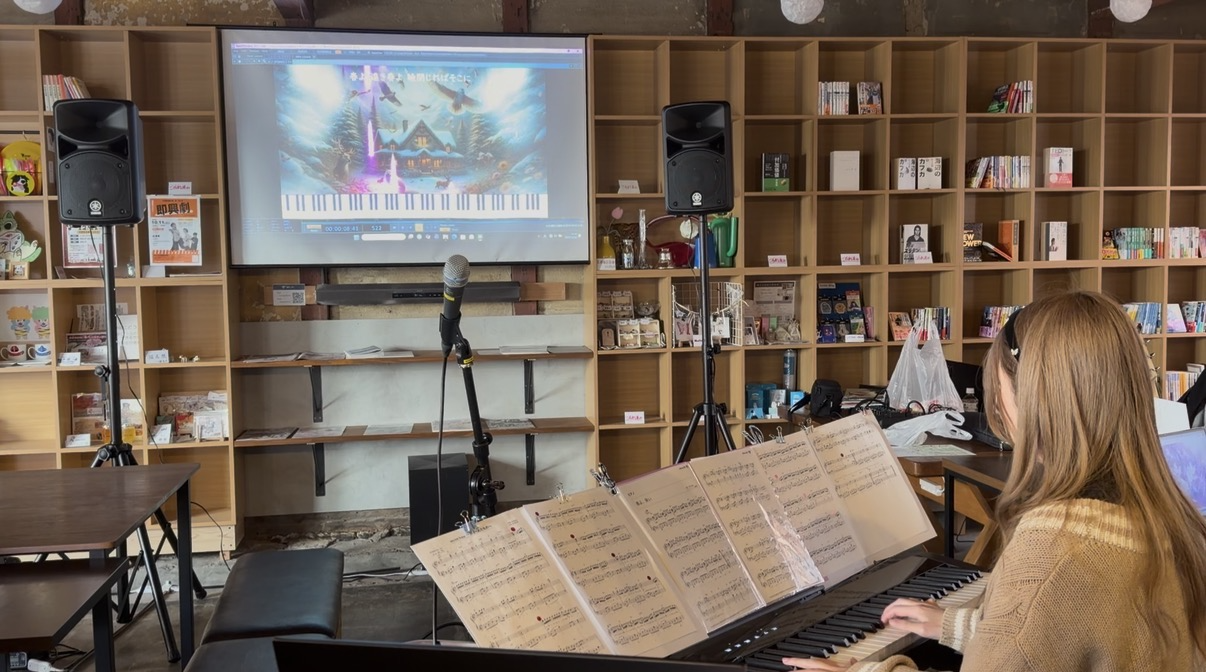
\includegraphics[width=\linewidth]{fig/2026-f17.png}
    \caption{実演の様子}
    \label{fig:sample17}
\end{figure}

%2.3
\subsection{評価と考察}
テスト演奏の結果，演奏者全員が概ね指定されたタイミングでフットペダル操作を行うことができ，
本システムの操作方法が事前説明と目印提示の条件下で適切に理解・実行されることが確認された．
特に，ピアノ演奏に一定の習熟を持つ演奏者は，演奏を中断することなくスムーズにペダル操作を行い，
演奏と映像操作を無理なく両立できていた．
また，被験者および観察者からは，テンポを厳密に意識せずとも音楽と映像が自然に一致している
との評価が得られた．以上より，本手法は演奏者の判断による操作を中心とした設計により，
演奏表現や即興性を損なうことなく映像演出を付加できる有効な代替手法であると考えている．
